\chapter{Cayley Diagrams}
\label{chapter:cayley_diagrams}
\thispagestyle{empty}

Recall that in the previous chapter we defined a group to be a set of actions that satisfies the following rules.

\begin{description}
\item[Rule 1.] There is a predefined list of actions that never changes.
\item[Rule 2.] Every action is reversible.
\item[Rule 3.] Every action is deterministic.
\item[Rule 4.] Any sequence of consecutive actions is also an action.
\end{description}

It is important to point out that this is an intuitive starting point and does not constitute the official definition of a group.  We'll continue to postpone a rigorous definition in this chapter and instead we will focus on developing more intuition about what groups are and what they ``look like."  

To get started, let's continue thinking about the game Spinpossible (see Chapter~\ref{chapter:intuitive_approach_groups}).  In Exercise~\ref{exer:number_spinpossible_boards}, we discovered that there are a total of $2^9\cdot 9! = 185,794,560$ possible scrambled Spinpossible boards.  Now, imagine we wanted to write a solution manual that would describe how to solve all these boards.  There are likely many possible ways to construct such a solution manual, but here is one way.  

The manual will consist of $185,794,560$ pages such that each page lists a unique scrambling of the $9\times 9$ board.  Don't forget that one of these scramblings is the solved board.  Let's make this page 1.  Also, imagine that the book is arranged in such a way that it isn't too difficult to look up a given scrambled board.  On each page below the scrambled board is a table that lists all possible spins.  Next to each spin, the table indicates whether doing that particular spin will result in a board that is either closer to being solved or farther.  In addition, the page number that corresponds to the resulting board is listed next to each spin.

In most cases, there will be many spins that take us closer to the solved board.  Given a scrambled board, a solution would consist of following one possible sequence of pages through the book that takes us from the scrambled board to the solved board.  There could be many such sequences.  If we could construct such a solution manual, we would have an atlas or map for the game Spinpossible.  We could always say, ``We are here," and ``The solution is down one of these paths."

Note that even if we make a wrong turn (i.e., follow a page that takes a farther away from the solution), we can still get back on track by following page numbers that take us closer to the solved board.  In fact, we can always get flip back to the page we were on before taking a wrong turn.  This page will be listed on our ``wrong turn page" since doing the same spin twice has the net effect of doing nothing.  If were to actually do this, the number of pages we would need to visit would be longer than an optimal solution, but we'd get to the solved board nonetheless.

Let's get a little more concrete.  Consider the game Spinpossible, except let's simplify it a little.  Instead of playing on the $9\times 9$ board, let's play on a $1\times 2$ board consisting of a single row with tiles labeled 1 and 2.  We'll refer to this simplified game as $\Spin_{1\times 2}$.  The rules of the game are what you would expect we are restricted to spins involving just the tiles in positions 1 and 2 of the original board.  A scrambling of $\Spin_{1\times 2}$ consists of any rearrangement of the tiles 1 and 2, where any of the tiles can be right-side-up or up-side-down.

\begin{exercise}
First, convince yourself that $\Spin_{1\times 2}$ satisfies our four rules of a group.
\begin{enumerate}
\item[(a)] How many scrambled boards are there for $\Spin_{1\times 2}$?  Don't forget to include the solved board.
\item[(b)] How many possible spins are there for $\Spin_{1\times 2}$?
\end{enumerate}
\end{exercise}

Let's try to make a map for $\Spin_{1\times 2}$, but instead of writing a solution manual, we will draw a picture of the group called a \textbf{Cayley diagram}.  The first thing we'll do is draw each of the scramblings that we found in the previous exercise.  It doesn't matter how we arrange all of these drawings, as long as there is some space between them.  These little drawings will form the vertices of our Cayley diagram.  Now, for each scrambling, figure out what happens when we do each of our allowable spins.  For each of these spins, we'll draw an arrow from the initial scrambled board to the resulting board.  Don't worry about whether doing each of these spins is a good idea or not.  In fact, figure out what happens when we do our allowable spins to the solved board, as well.  In this case, each of our scrambled boards will have 3 arrows heading out towards 3 distinct boards.  Do you see why?  

In order for us to keep straight what each arrow represents, let's color our arrows, so that doing a particular type of spin is always the same color.  For example, we could color the arrows that toggle the tile in the first position as green.  Recall that doing the same spin twice has the net effect of doing nothing, so we should just make all of our arrows point in both directions.

To make sure you are keeping up to speed, consider the following scrambled board.

\begin{center}
\begin{tikzpicture}[every node/.style={minimum size=.65cm}]
  \node [draw] (1) {\rotatebox{180}{$\underline{1}$}};
  \node [draw, right=0cm of 1] (2) {\rotatebox{180}{$\underline{2}$}};
\end{tikzpicture}
\end{center}

This board is one of our 8 possible scrambled boards in $\Spin_{1\times 2}$.  We have three possible spins we can do to this board: toggle position 1, toggle position 2, or spin the whole board.  Each of these spins has a corresponding two-way arrow that takes us to three different scrambled boards.  The figure below depicts the chunk of the Cayley Diagram involved the board above.  (I'll replace my hand drawn version later.)

\begin{center}
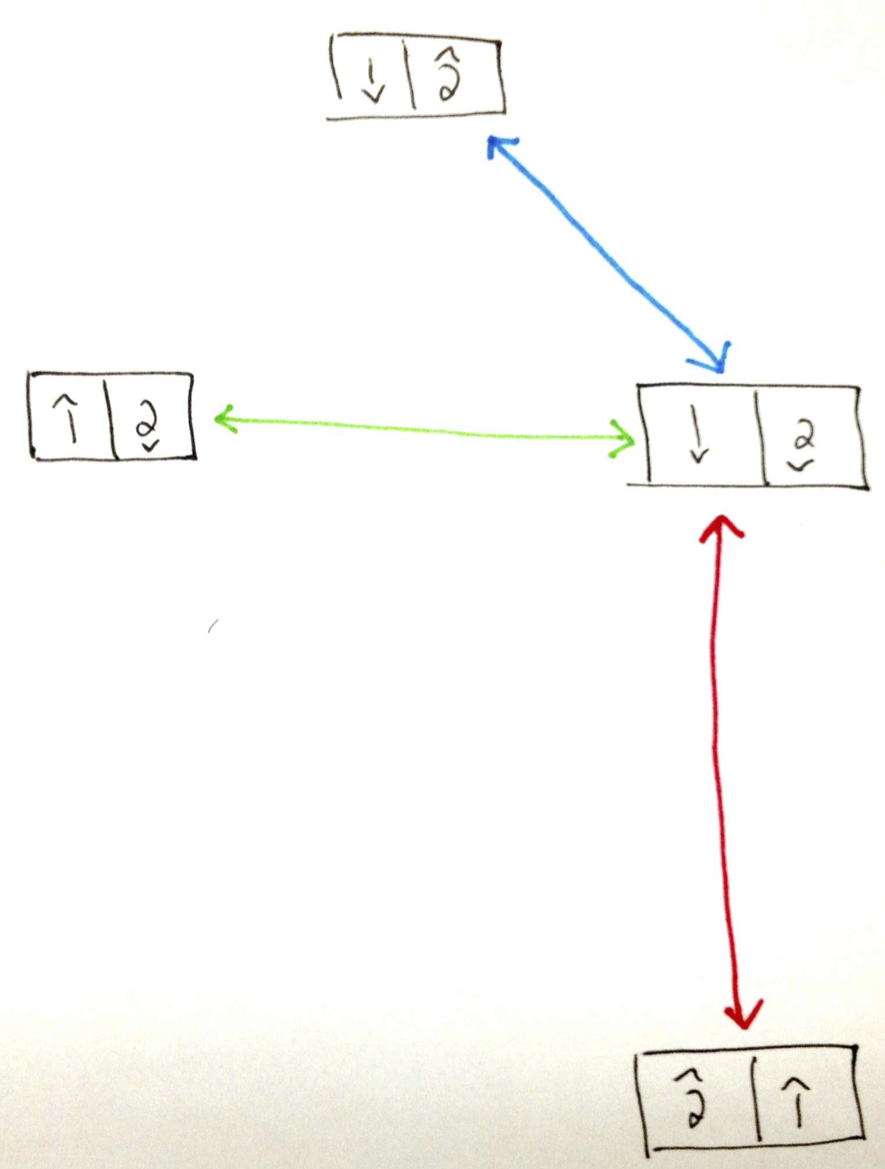
\includegraphics[width=2in]{chunk_cayley_spin1by2.png}
\end{center}

\noindent Notice we have three different colored arrows.  Can you see what each of the colors corresponds to?  If we include the rest of the scrambled boards and all possible spins, we obtain the complete Cayley diagram for $\Spin_{1\times 3}$.  (I'll replace my hand drawn version later.)

\begin{center}
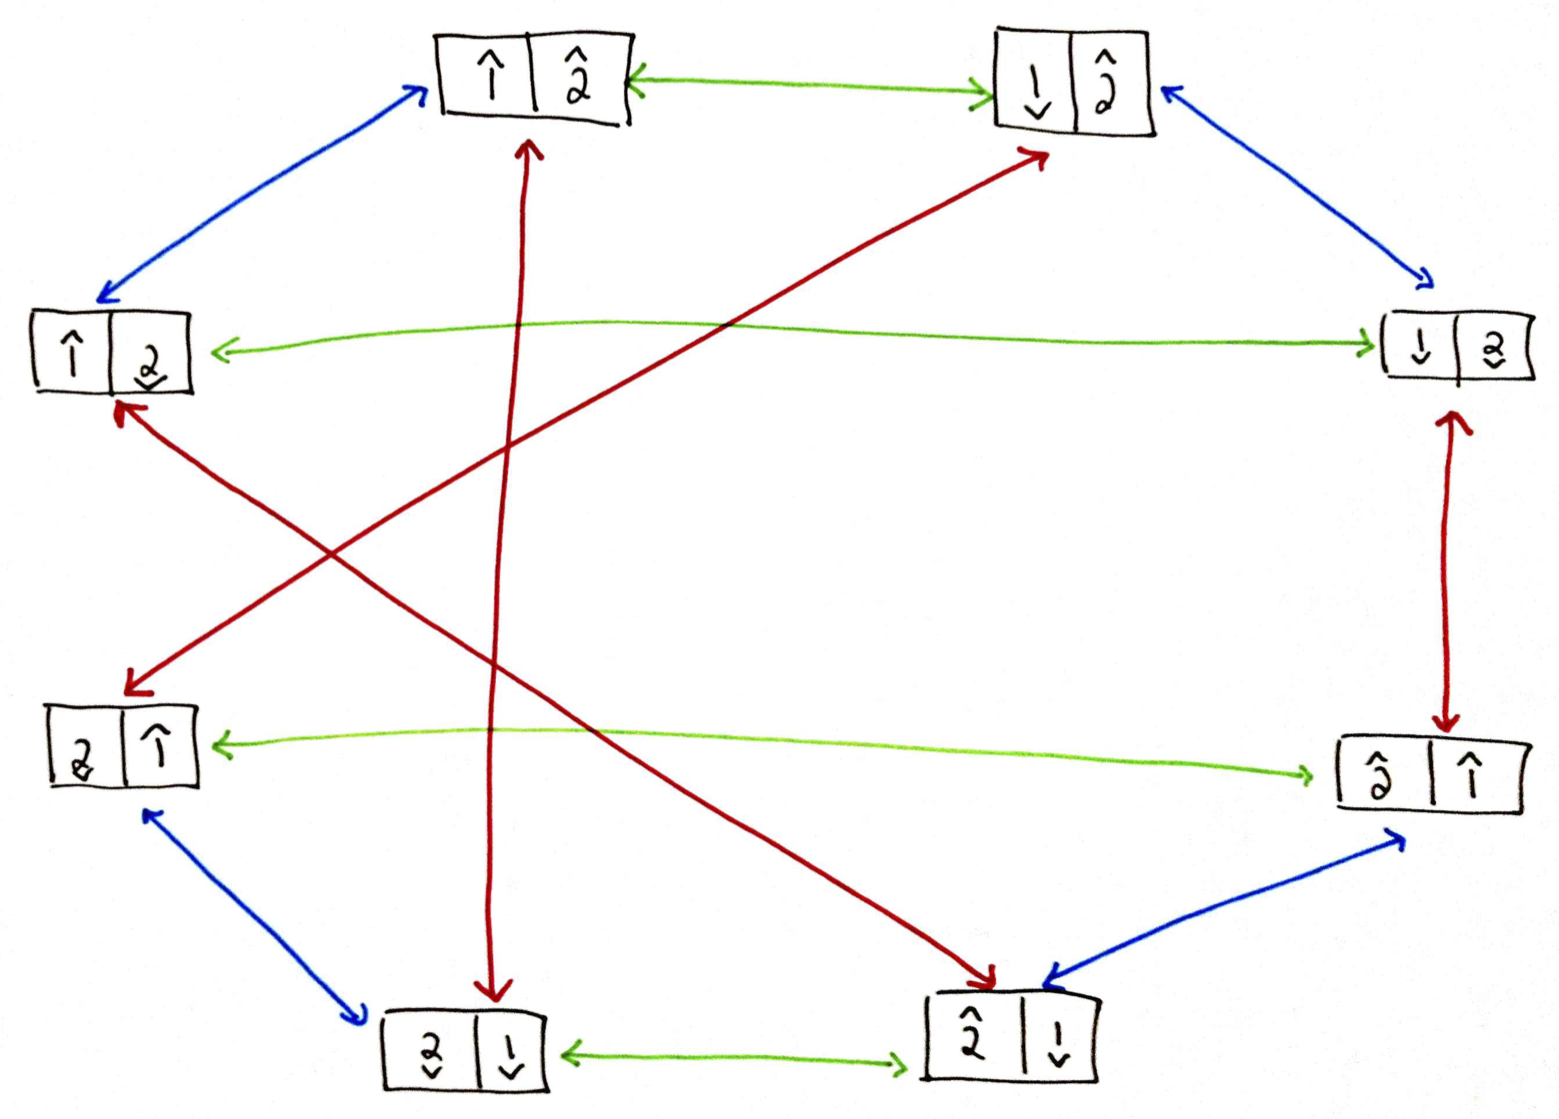
\includegraphics[width=4in]{cayley_spin1by2.png}
\end{center}

\noindent In this case, the spins that correspond to the three arrow colors are the \textbf{generators} of $\Spin_{1\times 2}$.  What this means is that we can obtain all possible scramblings/unscramblings by using just these 3 spins.  In other words, each of the scramblings corresponds to a word in these three spins.  The question remains as to whether we want each board to correspond to a word that unscrambles to the solve board or scrambles the solved board.  This might seem counter to how you want it to be, but we'll adopt the convention that each board corresponds to words that scramble the solved board into the desired scrambled board.

Let $t_1$ be the spin that toggles position 1, $t_2$ be the spin that toggles position 2, and $s_1$ be the spin that rotates the full board.  Recall that when we write down words, we should apply the actions from right to left (like function composition).  

Consider the following scrambled board.

\begin{center}
\begin{tikzpicture}[every node/.style={minimum size=.65cm}]
  \node [draw] (1) {{$\underline{2}$}};
  \node [draw, right=0cm of 1] (2) {\rotatebox{180}{$\underline{1}$}};
\end{tikzpicture}
\end{center}

\noindent Looking at our Cayley diagram for $\Spin_{1\times 2}$, we see that one way to get to this board from the solved board is to follow a blue arrow followed by a red arrow.  This corresponds to the word $s_1t_2$.  However, it also corresponds to the word $t_2s_1t_2t_1$ even though this is not an optimal solution.

\begin{exercise}
Given a word that corresponds to a scrambled board in the Cayley diagram for $\Spin_{1\times 2}$, how could we obtain a solution to the scrambled board?
\end{exercise}

\begin{exercise}
Using the Cayley diagram for $\Spin_{1\times 2}$, find three distinct words that correspond to the following scrambled board.  Don't worry about whether your word is of optimal length or not.

\begin{center}
\begin{tikzpicture}[every node/.style={minimum size=.65cm}]
  \node [draw] (1) {\rotatebox{180}{$\underline{1}$}};
  \node [draw, right=0cm of 1] (2) {\rotatebox{180}{$\underline{2}$}};
\end{tikzpicture}
\end{center}
\end{exercise}

\begin{exercise}
Consider the Cayley diagram for $\Spin_{1\times 2}$, but remove all the red arrows.  This corresponds to forbidding the spin that rotates the full $1\times 2$ board.  Can we obtain all of the scrambled boards from the solved board using only blue and green arrows?
\end{exercise}

\begin{exercise}
Repeat the previous exercise, but this time remove only the green arrows.  What about the blue arrows?
\end{exercise}